% 2010 年天津卷文科第 11 题：圆内接四边形 ABCD，AB 与 DC 延长交于 P。
% 来源 PDF：普通高考/2010/2010天津文.pdf（上游勘误版），SHA-256 e6b06813e17b7c332b651b8784c8fab0fcad0c8666ea6032a2958917c55307c9。
% 原页：第 1 页（A3 四栏）第 2 栏下部，书页码 637。
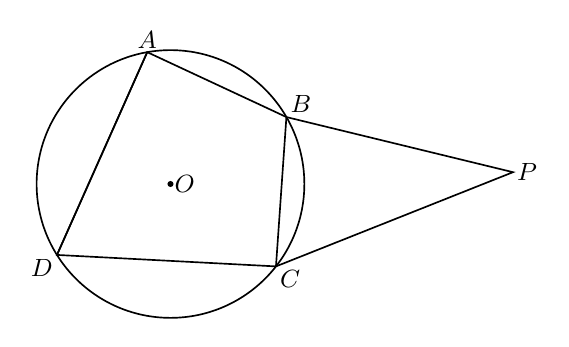
\begin{tikzpicture}[semithick, every node/.style={inner sep=1.2pt, font=\small}]
  \coordinate (O) at (0,0);
  \coordinate (A) at (100:1.7);
  \coordinate (B) at (30:1.7);
  \coordinate (C) at (-38:1.7);
  \coordinate (D) at (212:1.7);
  \coordinate (P) at (4.35,0.15);
  \draw (O) circle (1.7);
  \fill (O) circle (1.1pt);
  \node[right] at (O) {$O$};
  \draw (A) -- (B) -- (P) -- (C) -- (D) -- cycle;
  \draw (B) -- (C);
  \draw (A) -- (D);
  \node[above] at (A) {$A$};
  \node[above right] at (B) {$B$};
  \node[below right] at (C) {$C$};
  \node[below left] at (D) {$D$};
  \node[right] at (P) {$P$};
\end{tikzpicture}
